%%%%%%%%%%%%%%%%%%%%%%%%%%%%%%%%%%%%%%%%%
\documentclass[11pt]{scrartcl}
\usepackage[english]{babel}
\usepackage[utf8x]{inputenc}
\usepackage{amsmath}
\usepackage{graphicx}
\usepackage{DejaVuSerif}
\usepackage{DejaVuSans}
\usepackage{sourcecodepro}
\graphicspath{{Images/}}
\usepackage[colorinlistoftodos]{todonotes}
\usepackage{hyperref}
 \usepackage{float}

%\usepackage{fancyhdr}
%\pagestyle{fancy}

\areaset{17cm}{22.5cm}              % Set page width and height

\begin{document}
\begin{titlepage}
\pagenumbering{gobble}
\newcommand{\HRule}{\rule{\linewidth}{0.1mm}} 
\center % Center everything on the page
 

\textsc{Computer science engineering}\\[0.3cm] % heading course Number
\textsc{\Large Internet Of Things}\\[0.5cm] % heading course name
\textsc{\large Project n°1}\\[0.5cm] % Minor heading


\HRule \\[0.4cm]
{ \huge \bfseries Waste management system}\\[0.1cm] % Title of your Homework/assignment
\HRule \\[1.5cm]
 
%---------------------------------------------------------------------------------
%	AUTHOR SECTION (EDIT THE NAME and T.NO., only)
%---------------------------------------------------------------------------------

\begin{minipage}{0.4\textwidth}
\begin{flushleft} \large

Fabio \textsc{Codiglioni}\\ 919897 - 10484720  % Enter Your name and T.No.
\end{flushleft}
\begin{flushleft} \large


Alessandro \textsc{Nichelini}\\ 949880 - 10497404  % Enter Your name and T.No.
\end{flushleft}


\end{minipage}
\begin{minipage}{0.4\textwidth}
\begin{flushright} \large
\emph{Professor:} \\
Matteo \textsc{Cesana} % Supervisor's Name
\end{flushright}
\end{minipage}\\[1cm]
{\large \today}\\[1cm] % Date, change the \today to a set date if you want to be precise
\begin{figure}[H]
	\centering
	
\includegraphics[width=\textwidth,height=5.7cm,keepaspectratio]{resources/polimi_logo}% \\[0.5cm] % 
\end{figure}

\vfill % Fill the rest of the page with white-space

\end{titlepage}

\tableofcontents          % Required
\listoffigures
\newpage

\pagenumbering{arabic}

% Do not edit the below sections, enter all details in respective chapters
% Add the images/screen-shorts to the image folder and insert them in the respective chapters
\section{Abstract}
\subsection{General description}
This document describes the implementation of our project for the IoT course.
\\\\We decided to implement the project number 1: "\textit{Waste management system}". We used Contiki as the operating system for the IoT devices and Cooja as the simulator. We also used Node-RED to make data available to the external world and to build a lite dashboard to display system status and transmitted messages.
\\\\We implemented all requested requirements by writing two different firmwares: one for the bins and one for the truck. We manually built the requested node layout in Cooja simulator and we randomly generated a second layout.
\\\\Full source code is available at our repo: \url{https://github.com/fabiocody/CodiglioniNicheliniIoT}

\section{Implementation design choices}
\subsection{Architecture}
The system is composed by two firmwares:
\begin{itemize}
	\item \texttt{bin.c}
	\item \texttt{truck.c}
\end{itemize}
\texttt{bin.c} is the firmware to load on each smart bin. It is based on a finite state machine as shown in the picture below:

\begin{figure}[H]
	\centering
	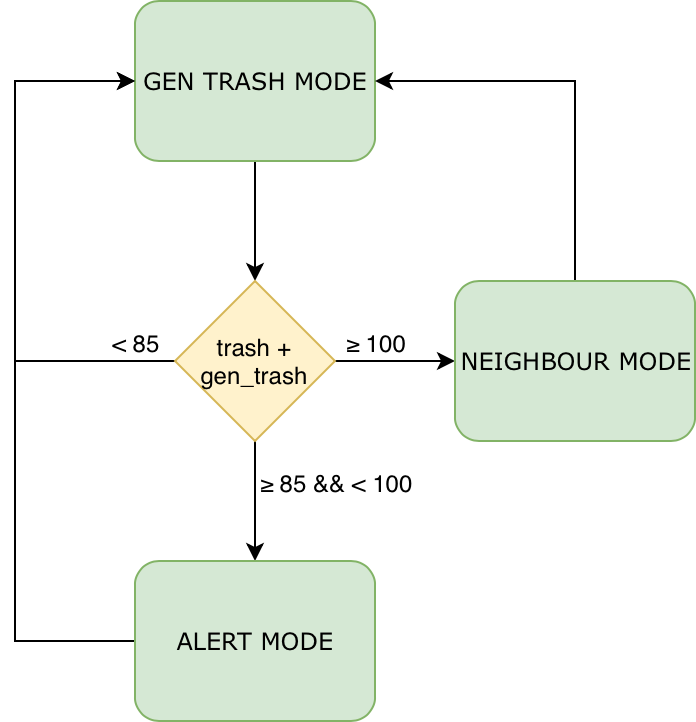
\includegraphics[width=0.5\textwidth]{resources/bin_state_chart}	
	\caption{Finite state machine model for bin.c}
\end{figure}

In particular all the operations and details are shown in the following flow chart diagram.

\begin{figure}[H]
	\centering
	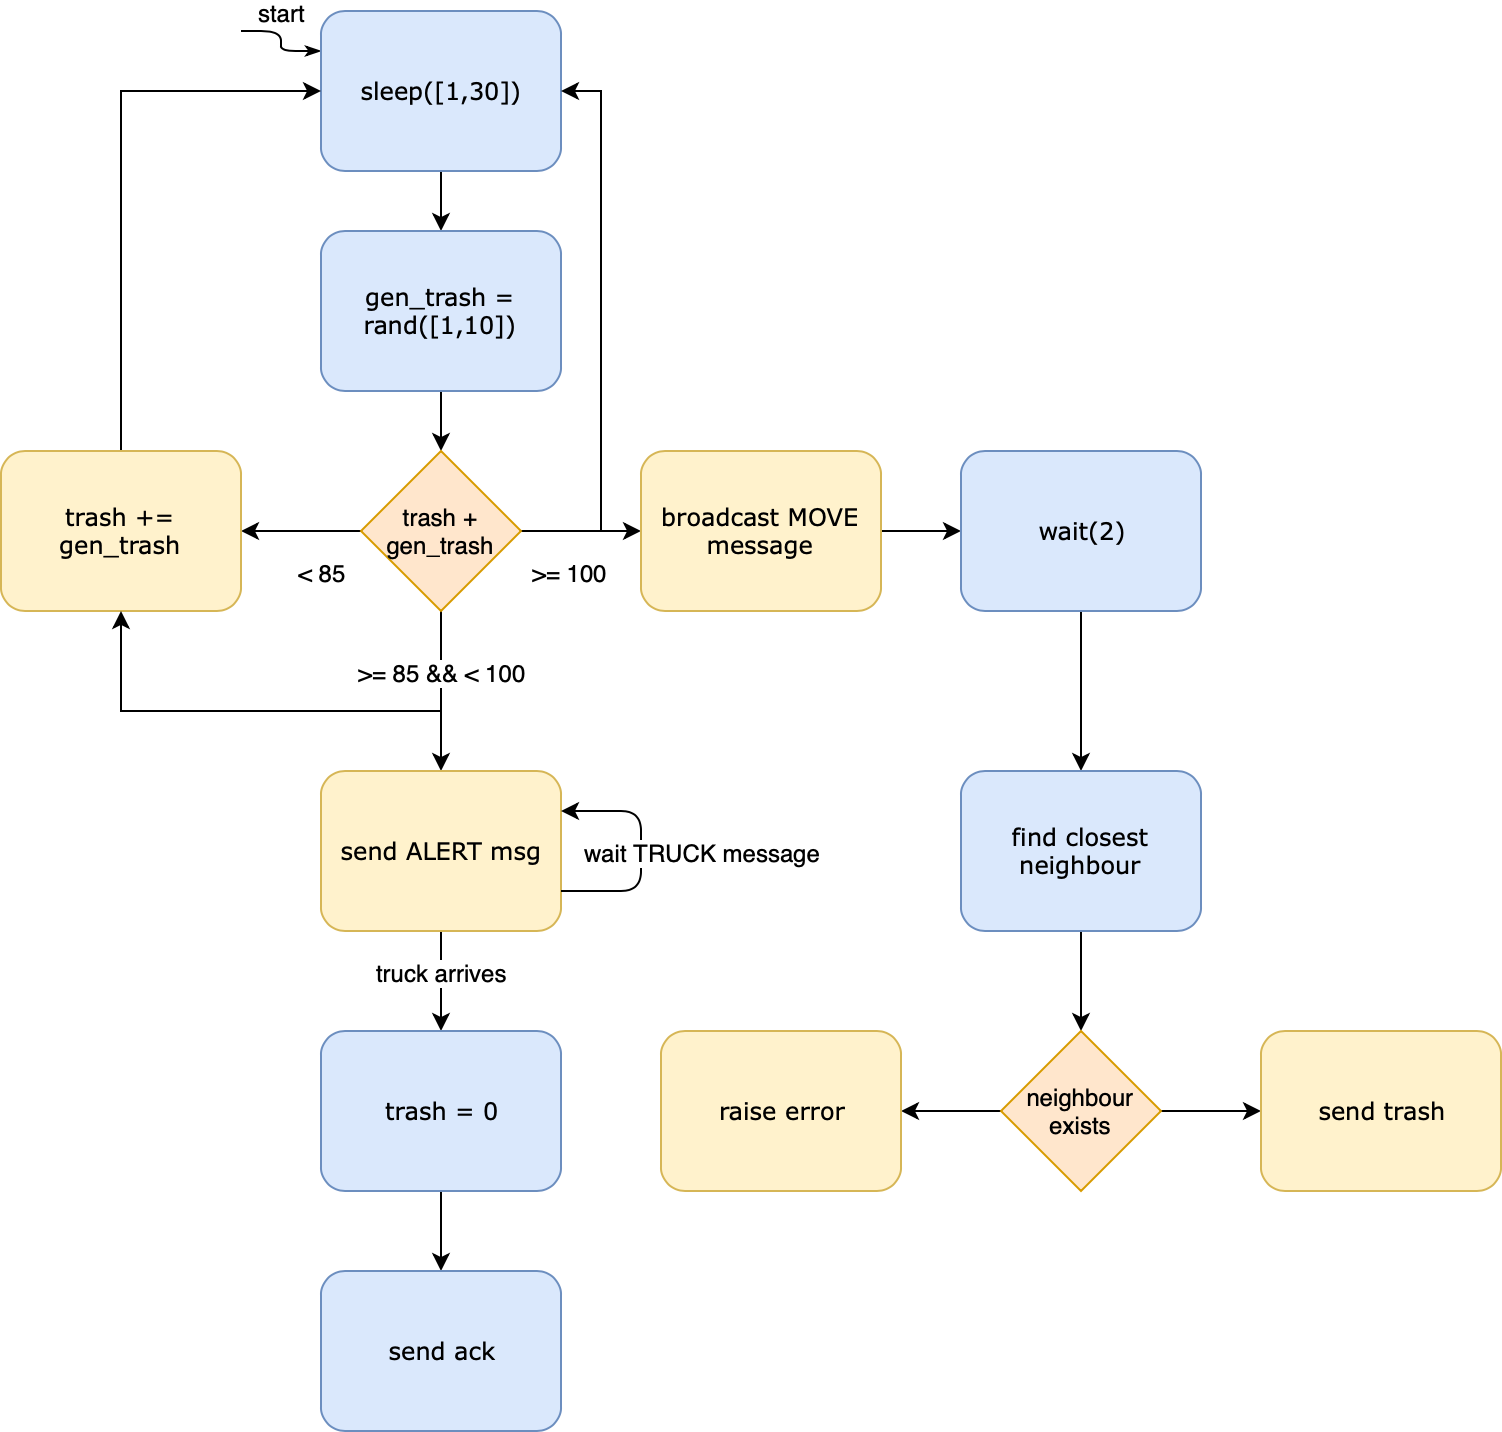
\includegraphics[width=0.7\textwidth]{resources/bin_flow_chart}
	\caption{Flow chart diagram for bin.c}
\end{figure}

\subsection{Other implementation details}

\begin{itemize}
	\item We adopted two different kind of transmission protocol (both of them based on native Rame stack):
		\begin{itemize}
			\item Broadcast:
			\item RUnicast:
		\end{itemize}
\end{itemize}








\end{document}
